%%%%%%%%%%%%%%%%%%%%%%%%%%%%%%%%%%%%%%%%%%%%%%%%%%%%%%%%%%%%%%%%%%%%%%%%%%%%%%%%%%%%%%%%%%%%%%%%%%%%%%%
%%													%%
%% 	DIPLOMOVÁ PRÁCE -  Návrh webového administrátorského rozhraní pro platformu GIS.lab			%%
%% 				 Tereza Kulovaná							%%
%%													%%
%% pro formátování využita šablona: http://geo3.fsv.cvut.cz/kurzy/mod/resource/view.php?id=775 	%%
%%													%%
%%%%%%%%%%%%%%%%%%%%%%%%%%%%%%%%%%%%%%%%%%%%%%%%%%%%%%%%%%%%%%%%%%%%%%%%%%%%%%%%%%%%%%%%%%%%%%%%%%%%%%% 

\documentclass[%
  12pt,         			% Velikost základního písma je 12 bodů
  a4paper,      			% Formát papíru je A4
  oneside,       			% Oboustranný tisk
  pdftex,				    % překlad bude proveden programem 'pdftex' do PDF
%%%  draft
]{report}       			% Dokument třídy 'zpráva'
%

\newcommand{\Fbox}[1]{\fbox{\strut#1}}

\usepackage[czech, english]{babel}	% použití češtiny, angličtiny
\usepackage[utf8]{inputenc}		% Kódování zdrojových souborů je UTF8

\usepackage[square,sort,comma,numbers]{natbib}

\usepackage{caption}
\usepackage{subcaption}
\captionsetup{font=small}
\usepackage{enumitem} 
\setlist{leftmargin=*} % bez odsazení

\makeatletter
\setlength{\@fptop}{0pt}
\setlength{\@fpbot}{0pt plus 1fil}
\makeatletter

\usepackage[dvips]{graphicx}   
\usepackage{color}
\usepackage{transparent}
\usepackage{wrapfig}
\usepackage{float} 

\usepackage{cmap}           
\usepackage[T1]{fontenc}    

\usepackage{textcomp}
\usepackage[compact]{titlesec}
\usepackage{amsmath}
\addtolength{\jot}{1em} 

\usepackage{chngcntr}
\counterwithout{footnote}{chapter}

\usepackage{acronym}

\usepackage[
    unicode,                
    breaklinks=true,        
    hypertexnames=false,
    colorlinks=true, % true for print version
    citecolor=black,
    filecolor=black,
    linkcolor=black,
    urlcolor=black
]{hyperref}         

\usepackage{url}
\usepackage{fancyhdr}
%\usepackage{algorithmic}
\usepackage{algorithm}
\usepackage{algcompatible}
\renewcommand{\ALG@name}{Pseudokód}% Update algorithm name
\def\ALG@name{Pseudokód}

\usepackage{dirtree}
\usepackage{booktabs}
\usepackage{graphicx}
\usepackage[table,xcdraw]{xcolor}

\usepackage[
  cvutstyle,          
  diploma           
]{thesiscvut}


\newif\ifweb
\ifx\ifHtml\undefined % Mimo HTML.
    \webfalse
\else % V HTML.
    \webtrue
\fi 

\renewcommand{\figurename}{Obrázek}
\def\figurename{Obrázek}

%%%%%%%%%%%%%%%%%%%%%%%%%%%%%%%%%%%%%%%%%%%%%%%%%%%%%%%%%%%%%%%%%
%%%%%%%%%%% Definice informací o dokumentu  %%%%%%%%%%%%%%%%%%%%%
%%%%%%%%%%%%%%%%%%%%%%%%%%%%%%%%%%%%%%%%%%%%%%%%%%%%%%%%%%%%%%%%%

%% Název práce
\nazev{Rozšíření zásuvného modulu QGIS pro zpracování GTFS o vizualizaci tarifních pásem PID }
{QGIS GTFS Plugin extension with visualization of PID tariff zones }

%% Jméno a příjmení autora
\autor{Bc.~Martin}{Kouba}

%% Jméno a příjmení vedoucího práce včetně titulů
\garant{Ing.~Martin~Landa,~Ph.D.}

%% Označení programu studia
\programstudia{Geodézie a~kartografie}{}

%% Označení oboru studia
\oborstudia{Geomatika}{}

%% Označení ústavu
\ustav{Katedra geomatiky}{}

%% Rok obhajoby
\rok{2021}

%Mesic obhajoby
\mesic{červen}

%% Místo obhajoby

\misto{Praha}

%% Abstrakt
%\abstrakt {slova}

%% Klíčová slova
\klicovaslova
{Python, QGIS, zásuvný modul, GTFS, PyQGIS}
{Python, QGIS, plugin, GTFS, PyQGIS}

%%%%%%%%%%%%%%%%%%%%%%%%%%%%%%%%%%%%%%%%%%%%%%%%%%%%%%%%%%%%%%%%%%%%%%%%

%%%%%%%%%%%%%%%%%%%%%%%%%%%%%%%%%%%%%%%%%%%%%%%%%%%%%%%%%%%%%%%%%%%%%%%%
%% Nastavení polí ve Vlastnostech dokumentu PDF
%%%%%%%%%%%%%%%%%%%%%%%%%%%%%%%%%%%%%%%%%%%%%%%%%%%%%%%%%%%%%%%%%%%%%%%%
\nastavenipdf
%%%%%%%%%%%%%%%%%%%%%%%%%%%%%%%%%%%%%%%%%%%%%%%%%%%%%%%%%%%%%%%%%%%%%%%

%%% Začátek dokumentu
\begin{document}

\catcode`\-=12  % pro vypnuti aktivniho znaku '-' pouzivaneho napr. v \cline 

% aktivace záhlaví
\zahlavi

% předefinování vzhledu záhlaví
\renewcommand{\chaptermark}[1]{%
	\markboth{\MakeUppercase
	{%
	\thechapter.%
	\ #1}}{}}

% Vysázení přebalu práce
%\vytvorobalku

% Vysázení titulní stránky práce
\vytvortitulku

% Vysázení listu zadani
\stranka{}%
	{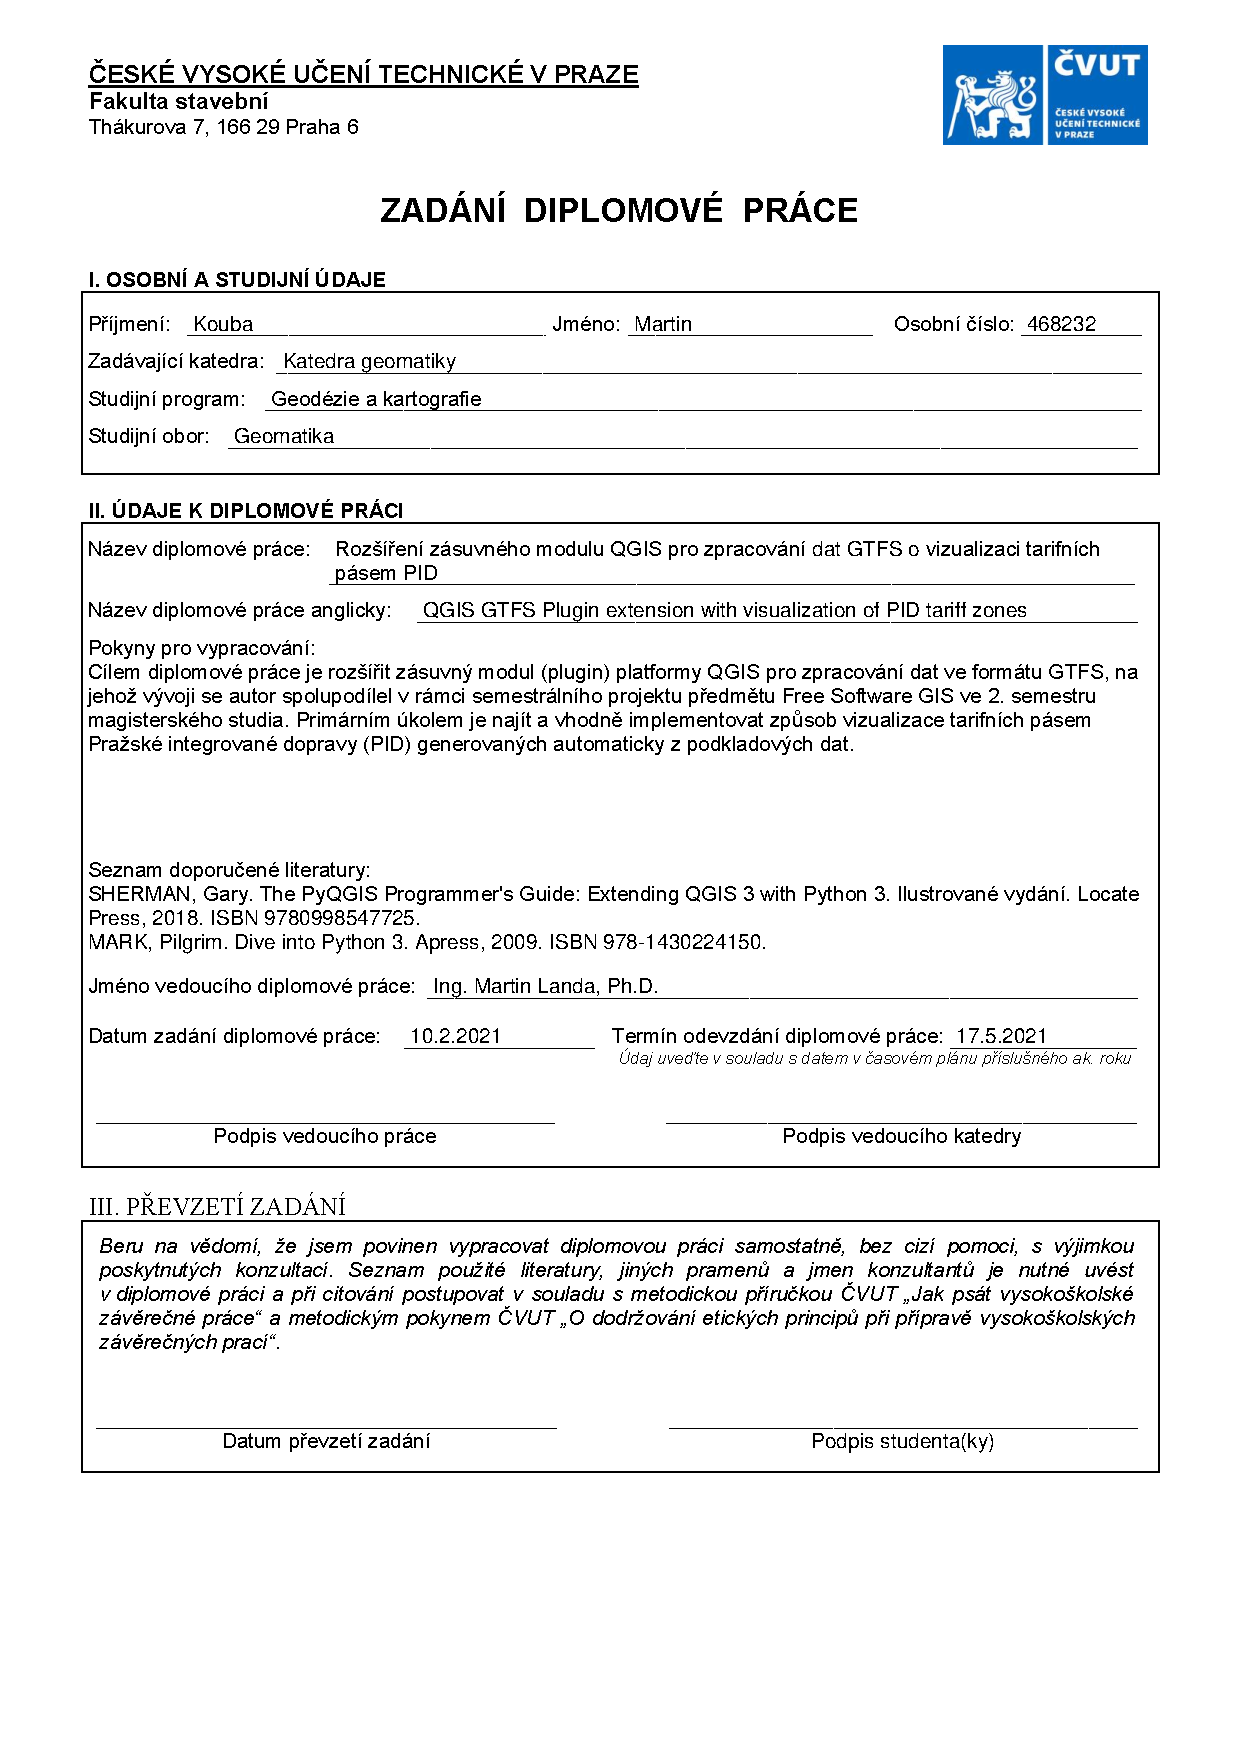
\includegraphics[scale=0.7]{../zadani/zadanidp.pdf}}%\sffamily\Huge\centering\ }%ZDE VLOŽIT LIST ZADÁNÍ}%
	%{\sffamily\centering Z~důvodu správného číslování stránek}

% Vysázení stránky s abstraktem
\vytvorabstrakt

% Vysázení prohlaseni o samostatnosti
\vytvorprohlaseni

% Vysázení poděkování
\stranka{%nahore
       }{%uprostred
       }{%dole
       \sffamily
	\begin{flushleft}
		\large
		\MakeUppercase{Poděkování}
	\end{flushleft}
	\vspace{1em}
		%\noindent
	\par\hspace{2ex}
	{Tímto bych chtěl poděkovat panu Ing. Martinu Landovi, Ph.D. za pomoc při …………………………………
	Zvlášť bych chtěl poděkovat celé své rodině …………………………………………
}
}

% Vysázení obsahu
\obsah

% Vysázení seznamu obrázků
\seznamobrazku

% Vysázení seznamu tabulek
\seznamtabulek

% jednotlivé kapitoly
\include{0-reserse}
%\include{1-uvod}
\chapter{GTFS}
\label{2-teorie-gtfs}

General Transit Feed Specification, zkráceně GTFS, je dokument, který definuje
obecný formát pro jízdní řády veřejné dopravy a příbuzné geografické informace.
GTFS „feeds“ umožňují veřejným dopravním agenturám zveřejňovat svá přepravní
data a vývojářům psát aplikace, které tato data spotřebovávají interoperabilním
způsobem neboli vícesystémovým mezinárodním provozuschopným způsobem. \cite{gtfs-info}

\section{Historie GTFS}
V Portlandu ve státě Oregon v USA se společnost TriMet pokusila jako jedna z prvních 
řešit problém s plánováním tranzitní dopravy pomocí otevřených dat sdílených širokou veřejností.
V roce 2005 společnost TriMet oslovila společnost Google s dotazem, zda mají nějaké plány
na začlenění tranzitní dopravy do svých plánovačů výletů na základě veřejných údajů TriMet.
Google jim kladně odpověděl a spojily síly s implementací jednoho z prvních plánovačů výletů v Portlandu.

Jedním z prvních problémů, kterým TriMet a Google čelily, byl problém udržitelných dat
- pro zajištění kvalitních cest by plánovač cest potřeboval přepravní řád, 
trasu a údaje o zastávkách v elektronickém formátu, který by byl neustále aktuální. 
Společnost TriMet ve spolupráci se společností Google naformátovala svá přepravní 
data do snadno udržovatelného a spotřebního formátu, který lze importovat do Map Google. 
Tento formát dat přepravy se stal známým jako Specifikace zdroje Google Transit (anglicky
Google Transit Feed Specification (GTFS)). 
V roce 2005 byla tato služba plánování cesty spuštěna jako Google Transit.

Od tohoto roku se GTFS stal nejpopulárnějším datovým formátem pro přepravní služby na světě. 
Spousta agentur se rozhodla sdílet své GTFS údaje s veřejností, zatímco některé agentury 
zůstaly zdrženlivé a přístup k datům nechaly jen některým partnerům. Ke 2. prosinci 2019
uvádí OpenMobilityData 1233 poskytovatelů s veřejně přístupnými kanály GTFS,
z nichž 465 je ve Spojených státech. 

V důsledku inovací vývojářů třetích stran jsou data GTFS nyní využívána různými softwarovými aplikacemi
třetích stran k mnoha různým účelům, včetně plánování výletů, map, vytváření jízdních řádů, mobilních dat,
vizualizace, přístupnosti, analytických nástrojů pro plánování a informační systémy v reálném čase.
V roce 2010 byl název formátu GTFS změněn na General Transit Feed Specification,
aby přesně reprezentoval jeho použití v mnoha různých aplikacích mimo produkty Google. \cite{transitwiki} 
 
% doplnit něco o historii GTFS 

\section{GTFS dataset}
GTFS \uv{feed} nebo lépe jako GTFS dataset\footnote{kolekce dat, která by měla být publikována na permanentní URL adrese}
je ZIP soubor, který obsahuje CSV soubory.

CSV, \textit{Comma-separated values}, v překladu \textit{hodnoty oddělené čárkami}, je jednoduchý 
souborový formát určený pro výměnu tabulkových dat. Data jsou oddělována „oddělovačem“.
Ačkoli podle definice by měl být formát oddělen čárkami, oddělovač může být prakticky cokoli. 
Nejčastějšími oddělovači jsou právě čárky, středníky nebo mezery. CSV soubor se 
může upravovat v jakémkoliv textovém editoru.

\begin{figure}[H] \centering
    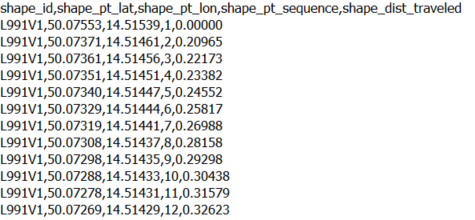
\includegraphics[width=250pt]{./pictures/ukazka-csv.PNG}
    \caption[Ukázka CSV formátu ze souboru shapes.txt]{Ukázka CSV formátu ze souboru shapes.txt}
	\label{fig:ukazka-csv}              
\end{figure}

V GTFS datasetu může být v současné době až 17 CSV souborů v textové podobě. Slovem \uv{může} je myšleno to,
že některé CSV soubory jsou požadované či podmíněně požadované a jiné volitelné.
Jaké CSV soubory obsahuje dataset záleží na konkrétním dopravním systému, který
tento dataset vytváří.

Termín \uv{požadované} znamená, že daný CSV soubor se musí nacházet v GTFS datasetu nebo dané pole
se musí nacházet v CSV souboru a v tomto poli musí být uvedena hodnota pro každý záznam. 

%přidat referenci na podmínky?
Termín \uv{podmíněně} požadované" znamená, že daný CSV soubor nebo pole je vyžadován za určitých podmínek, 
které jsou uvedeny v popisu souboru nebo pole. Mimo tyto podmínky je tento soubor nebo pole volitelný.

Termín \uv{volitelné} znamená, že daný CSV soubor nebo pole může být vynecháno. V případě zahrnutí 
volitelného pole mohou být některé položky prázdné řetězce, což je ekvivalentní s prázdným
polem.

V následující tabulce \ref{table:csv-soubory} jsou přehledně zobrazeny všechny CSV soubory,
které v současnosti v GTFS datasetu mohou být.

\newcolumntype{s}{>{\centering\arraybackslash\columncolor[HTML]{CCFFCC}} m{5cm}}
\newcolumntype{v}{>{\centering\arraybackslash\columncolor[HTML]{C4FFFD}} m{5cm}}

\begin{table}[h!]
\begin{center}
\begin{tabular}{ |s|v| } 
  \hline
  požadované/podmíněně požadované & volitelné \\ 
  \hline
  agency.txt & fare\_attributes.txt \\ 
  stops.txt & fare\_rules.txt \\ 
  routes.txt & shapes.txt \\
  trips.txt & frequencies.txt \\
  stop\_times.txt & transfers.txt \\
  calendar.txt & pathways.txt \\
  calendar\_dates.txt & levels.txt \\ 
  feed\_info.txt & translations.txt \\
  - & attributions.txt \\ 
  \hline      
\end{tabular}
\end{center}
\caption{Seznam CSV souborů v GTFS datasetu}
\label{table:csv-soubory}
\end{table}

Každý CSV soubor v GTFS datasetu má v prvním řádku názvy polí, do kterých je tento
soubor rozřazen. Jednotlivá pole mají různý datové typy, které jsou barva, kód měny, 
datum, email, enum (výčet), ID, kód jazyka, zeměpisná délka, zeměpisná šířka,
nezáporné číslo s plovoucí desetinnou čárkou, nezáporné celé číslo, telefonní číslo,
čas, text, časové pásmo a URL adresa.

Jedno z nejdůležitějších polí je pole s datovým typem ID, což je hodnota jednoznačně určující každý záznam.
Právě tento datový typ umožňuje propojení jednotlivých CSV souborů mezi sebou. ID může být
sekvence libovolných UTF-8 znaků. Pole s datovým typem ID se označují nakonci názvu s
\uv{\_id}. Na následujícím obrázku \ref{fig:GTFS-diagram} je toto propojení zobrazeno pomocí diagramu.

%přidat referenci na podmínky?
Na obrázku \ref{fig:GTFS-diagram} je taktéž tučně zobrazeno, které pole v daném CSV souboru
jsou požadované, podmíněně požadované nebo volitelné. 

\begin{figure}[H] \centering
    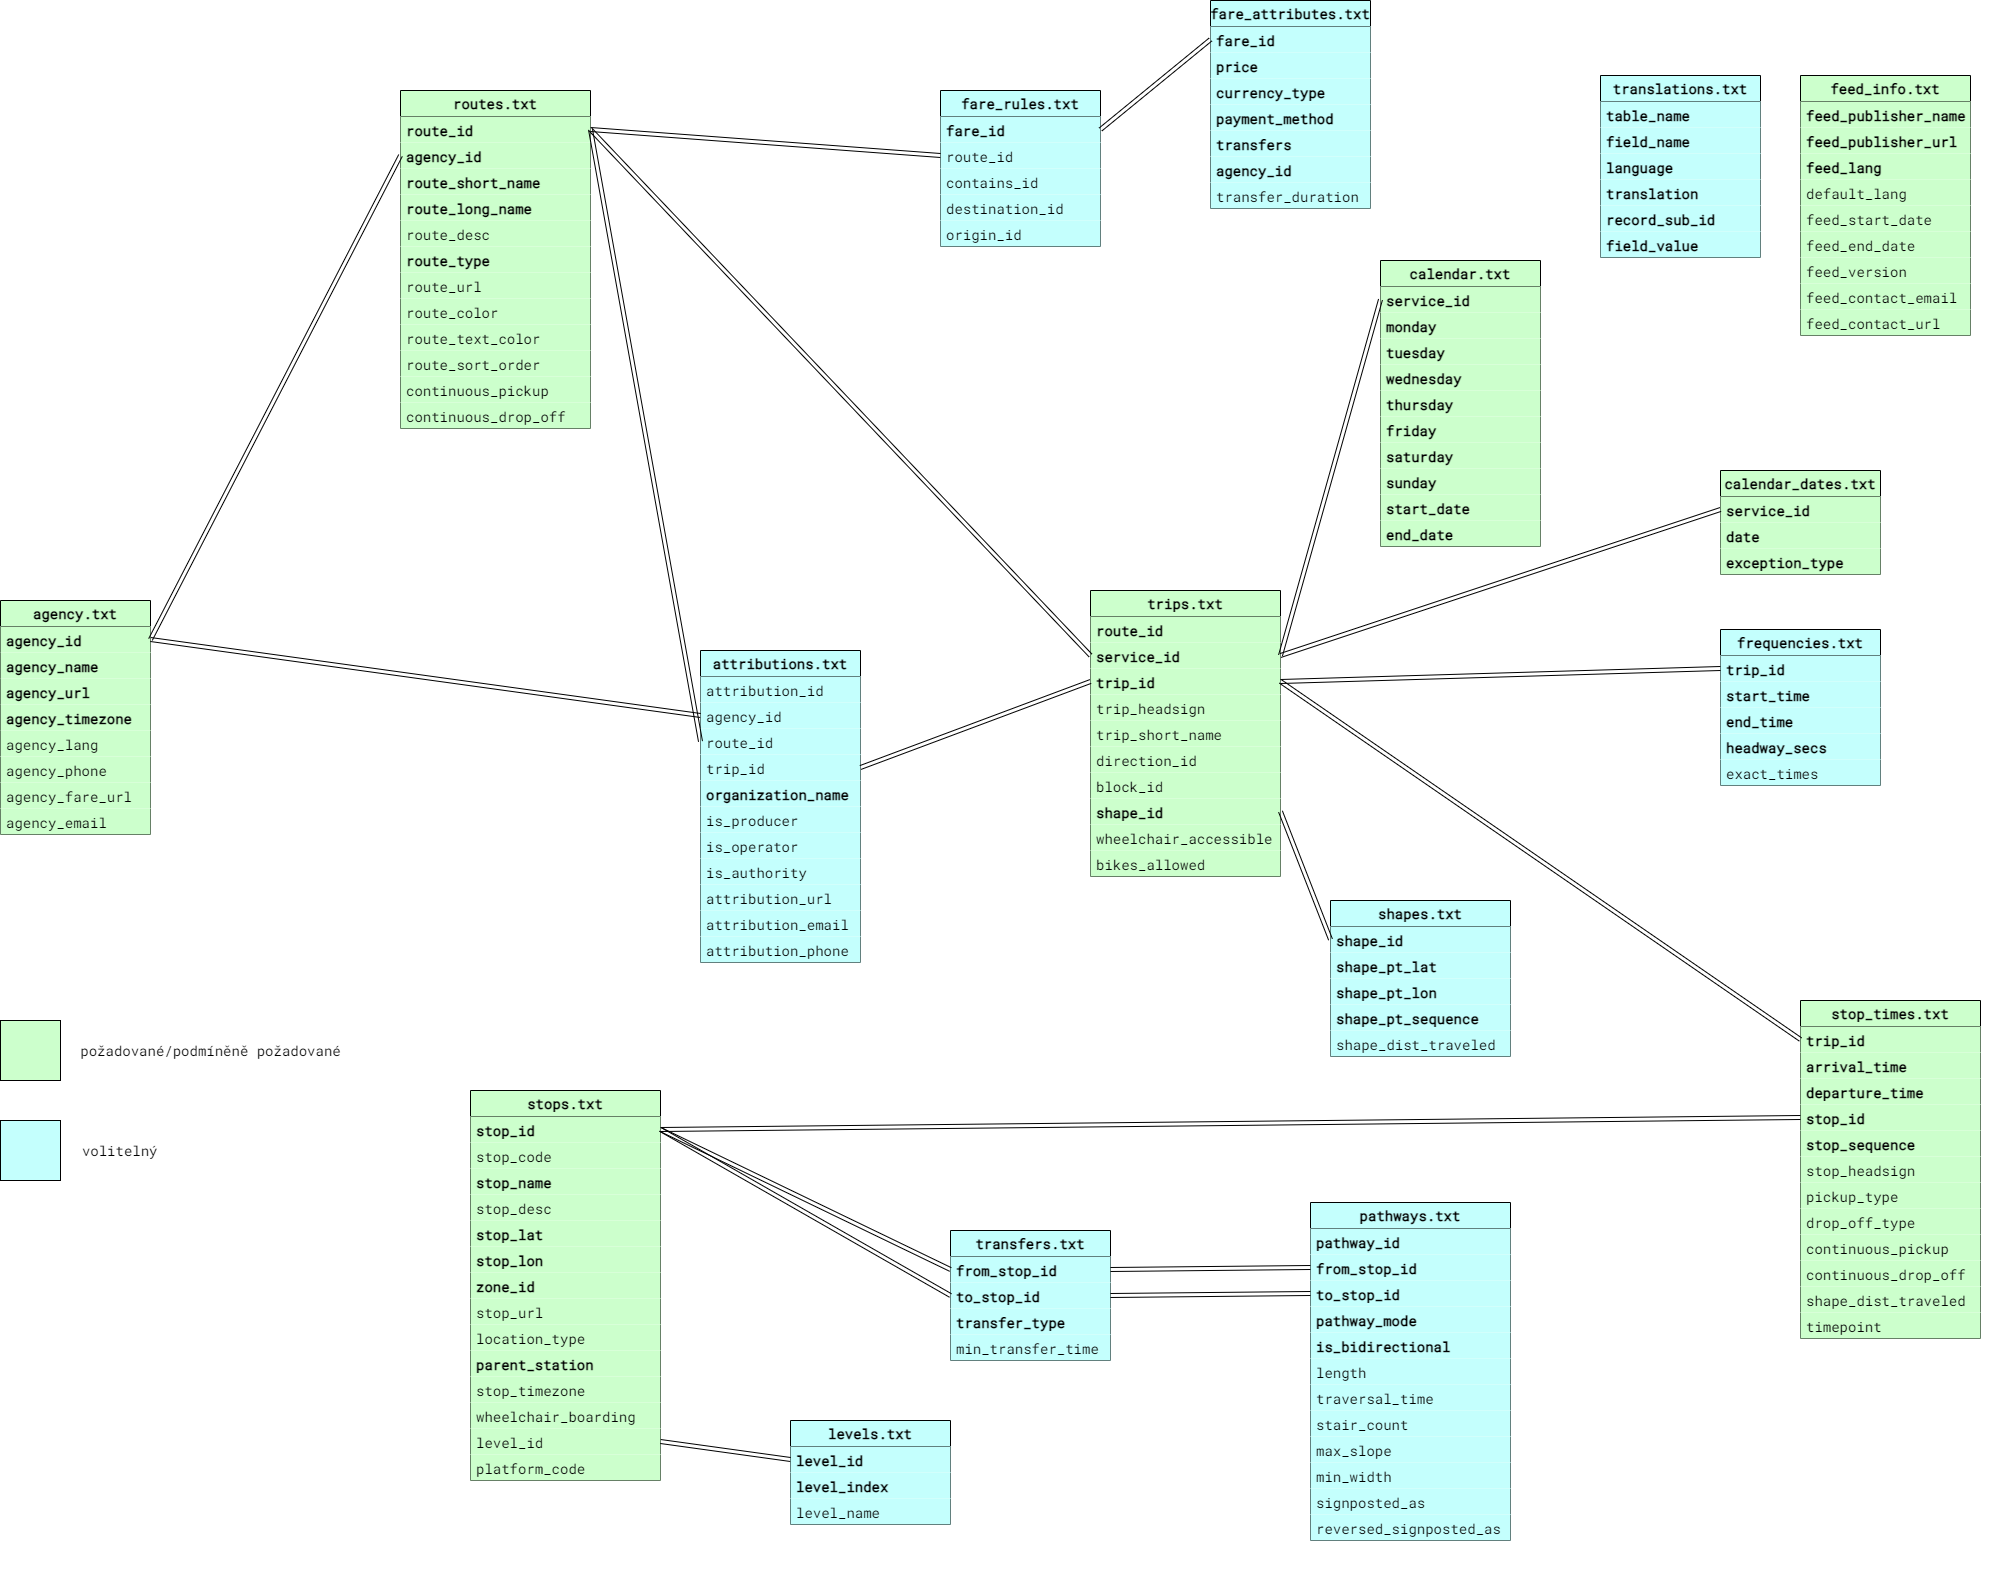
\includegraphics[width=400pt]{./pictures/GTFS-diagram.PNG}
    \caption[Diagram GTFS datasetu]{Diagram GTFS datasetu}
	\label{fig:GTFS-diagram}              
\end{figure}

Pro moji diplomovou práci byly dále důležité datové typy jako zeměpisná délka a zeměpisná šířka,
které již podle názvu obsahují zeměpisnou délku a šířku v souřadnicovém systému WGS84, barva zakódovaná 
jako šestimístné hexadecimální číslo, nezáporné číslo s plovoucí desetinnou čárkou a nezáporné celé číslo
nebo enum, což jsou předem definované konstanty.

\subsection{Soubor stops.txt}
\label{stops.txt}
Soubor \textit{stops.txt} se skládá ze 14 polí, z čehož 6 polí je požadovaných nebo podmíněně požadovaných 
a zbytek volitelných. Samotný soubor je požadovaný a měl by se nacházet v každém GTFS datasetu.

Prvním polem je vždy zpravidla \textit{stop\_id}, které je požadované a má datový typ ID.
Tato hodnota jednoznačně určuje každou zastávku. Pro PID\_GTFS, což je GTFS dataset Pražské integrované dopravy,
se pole \textit{stop\_id} skládá z kombinace písmen a čísel v souvislosti s typem spoje.

Druhým polem je volitelné pole \textit{stop\_code} v datovém typu text, což je krátký text nebo číslo, 
které identifikuje lokaci pro řidiče. 

Třetím polem je s datovým typem text \textit{stop\_name}. Jak už název napovídá, tak obsahuje název lokace. 
Je podmíněně požadované kvůli dalšímu volitelnému devátému poli \textit{location\_type} s datovým typem enum, 
které obsahuje druhy lokace.
Toto pole je definováno pomocí čtyř konstant:
\begin{itemize} 
\item 0 nebo prázdné - zastávka nebo nástupiště
\item 1 - železniční stanice 
\item 2 - vchod/východ ze železniční stanice 
\item 3 - místo ve stanici, které neodpovídá s žádnou z ostatních konstant z \textit{location\_type} 
\item 4 - specifické místo, kde lidé mohou nastoupit/vystoupit z vozidla
\end{itemize}

Čtvrtým polem je volitelné pole \textit{stop\_desc} v textovém datovém typu obsahující popis místa, 
které poskytuje užitečné a kvalitní informace.

Pátým a šestým polem je \textit{stop\_lat} a \textit{stop\_lon} s datovým typem zeměpisná šířka a délka
obsahující přesně tyto dvě hodnoty. Tyto dvě pole jsou podmíněně požadované kvůli poli \textit{location\_type}.

Sedmým polem s datovým typem ID je pole \textit{zone\_id}, které je pro tuto diplomovou práci obzvlášť důležité.
Je podmíněně požadované kvůli CSV souboru \textit{fare\_rules.txt}, pokud jsou v něm poskytovány informace o jízdném.
Pokud záznam v CSV souboru \textit{stops.txt} představuje stanici nebo vchod do stanice, je \textit{zone\_id} ignorováno.

Osmým polem je volitelný \textit{stop\_url} s URL adresou na webovou stránku o místě záznamu.

Deváté pole je \textit{location\_type} a bylo vysvětleno společně s třetím polem.

Desátým polem je podmíněně požadované pole \textit{parent\_station} opět kvůli propojení s polem \textit{location\_type}.
Má datový typ ID odkazující na pole \textit{stop\_id} a definuje hierarchii mezi různými místy definovanými v \textit{stops.txt}. 
a obsahuje ID nadřazeného umístění.

Poslední čtyři pole jsou volitelné. Prvním z nich je \textit{stop\_timezone} s datovým typem časového pásma,
\textit{wheelchair\_boarding} s datovým typem enum, které označuje, zda je z daného místa možné nastupovat na invalidní vozík.
Předposlední je \textit{level\_id} s datovým typem ID odkazující na soubor \textit{levels.txt} defi\-nující úroveň
umístění zastávky a poslední je \textit{platform\_code} s datovým typem text, 
což je identifikátor platformy pro zastávku patřící stanici.

Všechny tyto pole mají pevné pořadí a nesmí se přeházet. Na obrázku \ref{fig:stops} je ukázka CSV souboru \textit{stops.txt}
pro PID\_GTFS dataset, kde nejsou využívány všechny volitelné pole.

\begin{figure}[H] \centering
    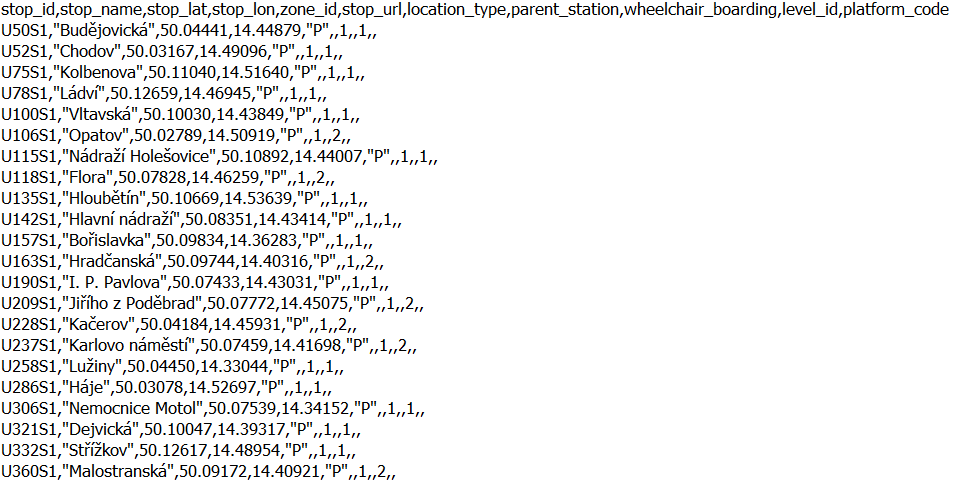
\includegraphics[width=400pt]{./pictures/stops.PNG}
    \caption[Ukázka CSV souboru stops.txt pro PID\_GTFS dataset]{Ukázka CSV souboru stops.txt pro PID\_GTFS dataset}
	\label{fig:stops}              
\end{figure} 
\chapter{Pražská Integrovaná doprava (PID)}
\label{3-teorie-pid}

Pražská integrovaná doprava (PID) je dopravní systém, který zahrnuje jak pozemní
dopravu (tramvaje, železnici, městské a příměstské autobusové linky, lanovou dráhu na Petřín),
tak i tu podzemní (metro). Tento dopravní systém zahrnuje i některé přívozy. 
Systém probíhá integrací společnými přepravními a tarifními podmínkami a jednotným dopravním řešením včetně 
koordinace jízdních řádů. \cite{pid}
\vskip 0.2in
 
\begin{figure}[H] \centering
    
\includegraphics[width=400pt]{./pictures/pid-logo.png}
    \caption[Logo Pražské integrované dopravy]{Logo Pražské integrované dopravy \cite{pid}}
	\label{fig:pid-logo}                                
\end{figure} 

\section{ROPID}

Chod integrace systému zajišťuje Regionální organizátor pražské integrované dopravy (zkráceně ROPID),
což je příspěvková organizace hlavního města Prahy. Jeho úloha je organizační a kontrolní
a ze své práce se odpovídá orgánům samosprávy a státní správy, které jej zabezpečením dopravy pověřily.

\begin{figure}[H] \centering
    
\includegraphics[width=200pt]{./pictures/ropid-logo.jpg}
    \caption[Logo ROPIDu]{Logo ROPIDu \cite{pid}}
	\label{fig:ropid-logo}                                
\end{figure}

ROPID se zabývá vytvářením, rozvíjení, a udržováním systému Pražské integrované dopravy v Praze a okolí,
včetně návazností na jiné systémy jako jsou Integrovaná doprava Plzeňského kraje,
Doprava Ústeckého kraje, Integrovaný dopravní systém Libereckého kraje nebo 
Integrovaná regionální doprava Královéhradeckého a Pardubického kraje.
Taktéž se zabývá vytvářením zásad a standardů dopravní obsluhy a jejich aplikace v závislosti
na dostupných finančních zdrojích a jejich projednání s obcemi, okresními úřady a dopravci.
ROPID výbírá dopravce, uzavírání smluv o závazku veřejné služby jménem města Prahy 
k zajištění provozu PID s dotčenými obcemi, Středočeským krajem a dopravci a kontrola jejich plnění.
Náplní ROPIDu jsou i organizace finančních toků v systému PID, návrh tarifu a jízdného v systému PID a
zajištění jednotnosti informačního systému PID.  \cite{wikipedia-ropid}

\section{Tarifní pásma PID}

Tzv. "tarifní pásma" je rozdělení Pražské integrované dopravy do určitých zón, kde v jednotlivých
zónách platí rozdílná cenové podmínky. Rozdělení tarifních pásem je následující:
P, 0, B, 1, 2, 3, 4, 5, 6, 7, 8, 9. Tarifní pásma P, 0 a B se nacházejí v Praze a územně
se spolu překrývají. Ostatní pásma (1 až 9) se nacházejí ve Středočeském kraji.

Do pásma P jsou zařazeny všechny linky metra, tramvají, městských autobusů, přívozů,
včetně lanové dráhy na Petřín a vybraných železničních stanic a zastávek v centru Prahy.
Pásmo P má dvojnásobnou tarifní hodnotu (tj. je počítáno jako dvě tarifní pásma).
Do pásma 0 jsou zařazeny dojezdové úseky příměstských autobusových linek a vybrané
železniční stanice a zastávky v širší oblasti okolo centra Prahy.
Do pásma B jsou zařazeny úseky příměstských autobusových linek a vybrané 
železniční stanice a zastávky v okrajových částech Prahy. 

Pro pásma nacházející se ve Středočeském kraji jsou zařazeny jednotlivé stanice 
a zastávky příměstských autobusových linek PID a vlaků zařazených do PID. 
Příslušnost stanice nebo zastávky k tarifnímu pásmu je vždy dána jízdním řádem konkrétní linky.\cite{pid}

\begin{figure}[H] \centering
    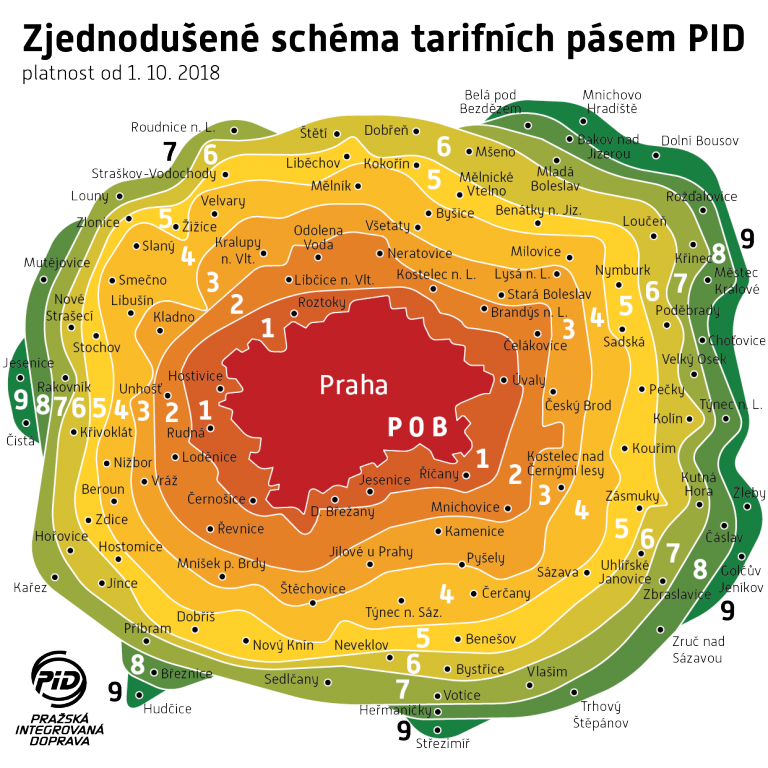
\includegraphics[width=400pt]{./pictures/pasma-schema.png}
    \caption[Schéma tarifních pásem PID]{Schéma tarifních pásem PID \cite{pid}}
	\label{fig:pasma-schema}                                
\end{figure}

\subsection{Tvorba tarifních pásem PID}

Tarifní pásma Pražské integrované dopravy se doposud tvoří manuálně. Zeptal jsem
se tedy paní Ing. Zuzany Šaškové z ROPIDu, která se tvorbou pásem zabývá, jakou metodiku
při tom používá. 

Paní Ing. Šašková používá na úpravu dat software ArcMap od společnosti Esri.
\textit{"Původní myšlenka při tvorbě tarifních pásem byla zohledňovat v mapě 
zastavěná území obce tak, aby je tarifní pásma pokud možno neprotínala,"} od této
myšlenky ustoupila kvůli náročnosti zpracování. \textit{"Dnes mám vytvořeny polygony 
jednotlivých pásem (nikoliv donuty), každé pásmo ručně upravím dle aktuálních změn."} 
V projektu při úpravách nepoužívá žádné sofistikované metody, jenom například obarvení
zastávek a jednotlivých polygonů tarifního pásma stejnou barvou, hraniční zastávek výraznou barvou 
případně pro následné úpravy. \textit{"Když ručně vytvaruji všechny polygony tak, aby procházely 
mezi zastávkami, které mají přiřazené jedno pásmo a skrz zastávky, které mají přiřazená dvě pásma, 
pustím si skript Pythonu, který z polygonů vyřeže donuty jednotlivých tarifních pásem a nakonec je spojí do jedné vrstvy."}

Takto paní Ing. Šašková upravuje tarifní pásma od dubna 2018 při každé úpravě zastávek. 
Zatímco dříve byla důležitá schématická verze mapy, v současnosti se připravuje on-line mapa PID, u které již je zapotřebí 
aby tarifní pásma odpovídala realitě a upravovala se v návaznosti na postup
integrace dalších oblastí Středočeského kraje do PID.

Zde na obrázku \ref{fig:pasma-schema} je uvedena nejstarší dochovaná podoba pásem z dubna roku 2018.
Pro zajímavost si lze všimnout, že v té době tarifní pásmo 7 bylo poslední a všechna pásma tvarově připomínala
spíše tu schématickou verzi.

\begin{figure}[H] \centering
    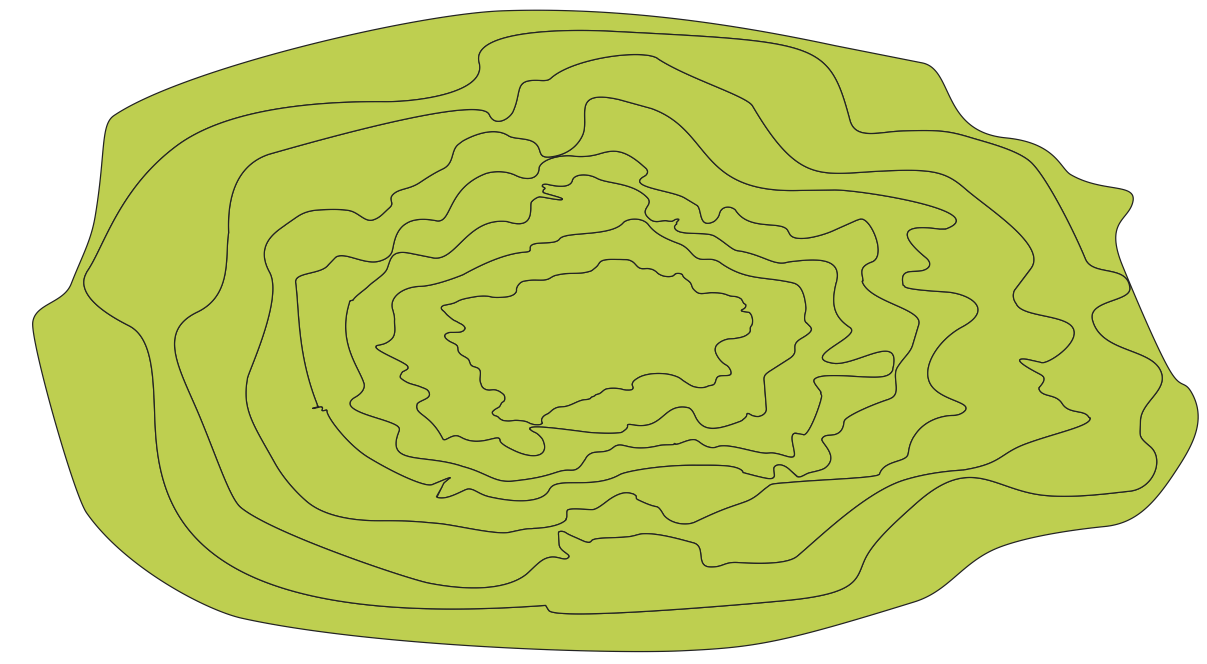
\includegraphics[width=400pt]{./pictures/pasma-nejstarsi.png}
    \caption[Nejstarší dostupná verze tarifních pásem PID]{Nejstarší dostupná verze tarifních pásem PID}
	\label{fig:pasma-schema}                                
\end{figure}




%\include{3-technologie}
%\include{4-praxe}
%\include{5-zaver}

% Vysázení seznamu zkratek
%
\begin{seznamzkratek}{ABCDE}      
	             	                   
      \novazkratka{CSV}
          {CSV}
          {Hodnota oddělená čárkami (Comma-separated values)} 
          
      \novazkratka{DPZ}	
	      {DPZ}
	      {Dálkový průzkum Země}  
          
      \novazkratka{GIS}
	      {GIS}
	      {Geografický informační systém (Geographic information system)}
          
      \novazkratka{GPKG}
	      {GPKG}
	      {Formát dat pro geografický informační systém (GeoPackage)}
          
	  \novazkratka{GUI}	
	      {GUI}
	      {Grafické uživatelské rozhraní (Graphical user interface)}
	               	             
	  \novazkratka{ID}	
	      {ID}
	      {Hodnota jednoznačně určující každý záznam} 	      	     
          
      \novazkratka{URL}
          {URL}
          {Jednotná adresa zdroje (Uniform Resource Locator)}                
          
      \novazkratka{WCS}	
	      {WCS}
	      {Web coverage service}
                                          
	  \novazkratka{WFS}	
	      {WFS}
	      {Web feature service}         
            
	  \novazkratka{WMS}	
	      {WMS}
	      {Webová mapová služba (Web map service)} 	

	  \novazkratka{WMTS}	
	      {WMTS}
	      {Služba webových mapových dlaždic (Web Map Tile Service)} 
          
      \novazkratka{ZIP}
          {ZIP}
          {Formát pro kompresi a archivaci dat} 	
          
	      	      
\end{seznamzkratek}

% Literatura
\nocite{*}
\def\refname{Odkazy}
\bibliographystyle{unsrt}
\bibliography{literatura}


% Začátek příloh
\def\figurename{Figure}%
\prilohy

% Vysázení seznamu příloh
\seznampriloh

%% Vložení souboru s přílohami
%\include{prilohy}

% Konec dokumentu
\end{document}
